
\chapter{Uvod} % Main chapter title

\label{Uvod} % For referencing 


%------------------------------------------------------------------------------

\section{Osnovni biološki i hemiski koncepti}

Svi živi organizmi sastoje se od jedne ili više ćelija a svaka ćelija od
molekula. Veliki \footnote{ Obično se molekulska masa od $1000 Da$ (Daltona) uzima kao 
granica između malih molekula i makromolekula.}
molekuli (makromolekuli) biološkog porekla obično \footnote{
  Lipidi recimo nisu polimeri ali su principijalno slični
} su sačinjeni od
ponavljajućih strukturnih jedinica \keyword{monomera} \textit{(mono- = jedan,
mer- = deo)}, međusobno povezanih \keyword{kovalentnim} vezama.  Takav molekul
zovemo \keyword{polimer} \textit{(poli- =mnogo, -mer= deo)}. 
% Polimer može da bude \textit{homo-polimer}, sačinjen od jednog tipa monomera
% ili suprotno \textit{hetero-polimer}, sačinjen od nekoliko raznih tipova
% monomera.
Skup monomera možemo da smatramo azbukom koja gradi jezik polimera.  Mali broj
monomera je dovoljan za strukturnu kompleksnost bilo koje ćelije.  Tri 
najznačajnija tipa bioloških polimera i njihovi monomeri prikazani su tableom \ref{tab:polimeri}.


\begin{table}[htpb]
  \centering
  \caption{Najznačajniji biološki polimeri}
  \label{tab:polimeri}
  \begin{tabular}{ll}
    \keyword{Polimer}            & \keyword{Monomer} \\
    Ugljeni hidrati              & Monosaharid (šećeri) \\
    Nukleinska kiselina (DNK)    & Nukleotid \\
    Protein                      & Aminokiselina \\
    \hline



  
  \end{tabular}
\end{table}



\subsection{Proteini}

Proteini su najčešći biološki makromolekuli koji čine i do $80\%$ suve mase
organizma.  Strukturno protein je linearan polimeri sačinjen od lanca
\keyword{aminokiselina}(monomeri). 



\section {Bioinformatičke baze podataka}

Automatizacija bioloških i hemiskih analliza početkom 21 veka omogućila je
ubrzanu i paralelnu analizu velikog broja uzoraka. Ove tehnologije žargonski su
poznate kao \keyword{tehnologije velike propusnosti} \en{high throughput
technology }. Primera radi tehnologije \keyword{sekvenciranja nove generacije}
\en{Next-Generation Sequencing} ili skraćeno \keyword{NGS} neprekidno napreduju
spuštajući cenu procedure i eksponencijalno povećavajući količinu dostupnih
sekvenci. Da bi se razumeo uticaj NGS tehnologije razmotrimo sledeći tok
informacija.  Od sveže sekvencionisanih nepoznatih genoma predviđaju se
potencijalni geni, od gena potencijalne proteinske sekvence.  Dobijene
proteinske sekvence mogu se dalje klasterovati u familije, automatski
anotirati, predviđati im se struktura itd.  Zatim moguće je vršiti analize za
generisanje novih bioloških znanja. Povezanost između funkcije i neuređenosti
proteina je jedan primer biološkog znanja. Dakle generisanje novih informacija
u jednoj oblasti (u ovom slučaju genomici) propagira se u druge oblasti
bioinformatike. Ovo je samo jedan primer ali ilustruje 2 bitne stvari.
\begin{enumerate}
  \item Informacije eksponencijalno rastu uvodeći čitavu oblast
    \keyword{omike}\footnote{termin objedinjuje gen\textbf{omiku}, proteomiku,
    transkriptomiku, glikomiku...} \en{omics}  u teritoriju \en{Big
  Data}\parencite{Chen2017}. U našem radu pažljivo su odabrani podaci malog
  obima kako bi se izbegao ovaj scenario i sve analize su urađene na klasičnom
  kućnom računaru.
  \item U bioinformatici podaci su jako povezani. 
\end{enumerate}

Povezanost podataka preslikava se na baze. Većina baza je usko specijalizovana
za jedan tip informacije ili jedan organizam, ali zato sadrži reference ka
drugim(spoljnim) bazama, naučnim radovima ili  manje formalnim ali
informativnim resursima (veb strane, vikipedija, itd...). Druge baze kao što je
UniProtKB, pored primarnog sadržaja održavaju i veliki broj referenci(dbxref)
pokušavajući da međusobno povežu sve dostupne informacije. Konkrentno
UniprotKB(feb. 2018) održava reference ka čak 164 različite
baze\footnote{\url{www.uniprot.org/docs/dbxref}}.
Dakle bioinformatika kao disciplina podrazumeva da će analize biti vršena
kombinacijom različitih baza.  Zbog raznovrsnosti i svrhe prikupljenih
informacija postoji veliki broj kategorija\footnote{Baze ne pripadaju
ekskluzivno samo jednoj kategoriji}(vrsta) baza.  Na adresi
\url{www.proteininformationresource.org/staff/chenc/MiMB/dbSummary2015.html}
kategorizovane su i prikazane kvalitenije proteinski orijentisane baza, ali
prikazana lista nipošto nije iscrpna\parencite{Chen2017}. Za naše istraživanje
dovoljno je poznavanje naredne tri kategorije:

\begin{itemize}
  \item Baze sekvenci.\\ 
        Ove baze teoretski sadrže sve poznate sekvence i kontrolišu dodeljivanje 
        identifikacionog broja sekvence.
    \begin{itemize}
      \item Proteinske sekvence (UniProtKB)
      \item DNK sekvence (EMBL, GenBank, DDBJ)
    \end{itemize}
  \item Baze strukture: PDB, DisProt, D2P2, MobiDB, PDB
  \item Baze homologija: Gene Ontology, Protein Ontology
\end{itemize}


\subsection{UniProtKB/Svis-Prot}


\keyword{UniProt} skraćeno od \en{Universal Protein Resource} je konzorcijum
nastao 2002 god. izmedju tri organizacije: Evropski Bioinformatički
Institut (EBI), Švajcarski institut za Bioinformatiku (SIB) i Resurs
Proteinskih Informacija(PIR).  ''Misija UniProt-a je da naučnoj zajednici
obezbedi sveobuhvatan, visokokvalitetan i slobodno dostupan resurs proteinskih
sekvenci i funkcionalnih informacija.''\footnote{\url{www.uniprot.org}} 


uniprot obuhvata nekoliko baza i podbaza sa striktno definisanim tokom
informacija \ref{fig:uniprot_overview}. Od prikazanih najbitnija je
\keyword{UniprotKB} \en{UniProt Knowledge Base} sačinjena od 2 podbaze.


\begin{enumerate}
  \item \keyword{Svis-Prot} \en{Swiss-Prot} sadrži visoko kvalitetne antoacije
    \keyword{ne redundantnih}\ref{} proteinskih sekvenci. Informacije o sekvenci su
    dobijene iz postojeće literature a kompjuterski predviđene anotacije su
    ručno proverene. Svis-Prot kao baza postoji preko 30 godina.

  \item TrEMBL \en{Translated EMBL} je nadskup Svis-Prot sekvenci čije čije su
    sekvence dobijene prevođenjem EMBL nukleinskih sekvenci ali još nisu stigle
    da budu ručno  proverene. Ove sekvence su redundantne i njihova obimnost
    posledica je masovne primene NGS tehnologija. U februaru 2018. god TrEMBLE
    sadržao je 107,627,435 sekvenci što je oko 200 puta više u poređenju sa
    556,568 ručno proverenih Svis-Prot sekvenci. Sve nove sekvence prvo ulaze u
    sastav TrEMBL da bi ručnom proverom napredovale u Svis-Prot što je donekle
    prikazano grafikom \ref{fig:uniprot_overview}.
\end{enumerate}


\begin{figure}[h!]
  \centering
  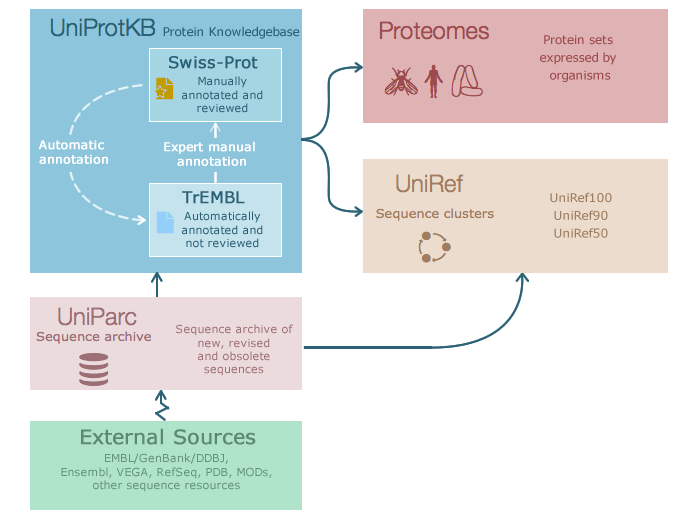
\includegraphics[width=0.8\linewidth]{uniprot_overview.png}
  \caption{Šematski prikaz povezanosti UniProt baza \ref{}}
  \label{fig:uniprot_overview}
\end{figure}

% Biological Databases:
% Sequence Databases
%   DNK: EMBL, GenBank, DDBJ (teoretski "sve" poznatne javne sekvence)
%        sadržaj se međusobno deli
%        jedine izdaju accession brojeve
% Genome Databases
% Structure Databases
%
% Minimum obaveznih informacija 
%   Sekvenca
%   identifikacioni broj (AC)
%   reference
%   taksonomija
%   ANNOTATION/CURATION
%   keywords
%   cross-references
%   documentation


Distribucije Svis-Prot baze dostupne su u nekoliko tekstualnih formata: ravna
datoteka \en{flat file}, XML, RDF/XML.  Ravni tekstualni format zbog
standardizacije prati format EMBL baze.  Unos u bazu se zove \keyword{slog}
\en{record} i sadrži sve informacije vezane za jedan protein. Jedan slog
ilustrovaćemo uprošćenim primerom u formatu ravne datoteke:

\lstset{ 
  basicstyle=\footnotesize\ttfamily,        % the size of the fonts that are used for the code
  captionpos=b,                    % sets the caption-position to bottom
  commentstyle=\color{mygreen},    % comment style
  deletekeywords={...},            % if you want to delete keywords from the given language
  escapeinside={\%*}{*)},          % if you want to add LaTeX within your code
  extendedchars=true,              % does not work with UTF-8
  keywordstyle=\color{blue},       % keyword style
  % language=Octave,                 % the language of the code
  morekeywords={ID, AC, PE, KW, GO, SQ}, % if you want to add more keywords to the set
  numbers=left,                    % where to put the line-numbers; 
  numbersep=5pt,                   % how far the line-numbers are from the code
  numberstyle=\color{mygray}, % the style that is used for the line-numbers
  % rulecolor=\color{black},         % if not set, the frame-color may be changed on line-breaks within not-black text (e.g. comments (green here))
  showstringspaces=false,          % underline spaces within strings only
}

\begin{lstlisting}
ID   ACSA_DROME              Reviewed;         670 AA.  | ime sloga, info
AC   Q9VP61; Q24226; Q8IH30; Q9VP60;                    | identifikacioni br.
DT   19-SEP-2003, integrated into UniProtKB/Swiss-Prot. | ulazak u Svis-Prot
DT   01-MAY-2000, sequence version 1.                   | ulazak u TrEMBL
DT   25-OCT-2017, entry version 116.                    | poslednje 
                                                          osvezavanje sloga
DE   RecName: Full=Acetyl-coenzyme A synthetase;        |
DE            EC=6.2.1.1;                               |
DE   AltName: Full=Acetyl-CoA synthetase;               |
DE            Short=ACS;                                |
GN   Name=AcCoAS; ORFNames=CG9390;                      |
OS   Drosophila melanogaster (Fruit fly).               | Taksonomija
OC   Eukaryota; Metazoa; Ecdysozoa; Arthropoda; Hexap...|
OC   Pterygota; Neoptera; Holometabola; Diptera; Brac...|
OC   Ephydroidea; Drosophilidae; Drosophila; Sophopho...|
OX   NCBI_TaxID=7227 {ECO:0000312|EMBL:AAL90278.1};     |
                                                        
RN   [1] {ECO:0000305}                                  | Prva referenca
RP   NUCLEOTIDE SEQUENCE (ISOFORM B).                   | 
RA   Russell S.R., Heimbeck G.M., Carpenter A.T., Ash...| Autori
RT   "A Drosophila melanogaster acetyl-CoA-synthetase...| Naslov
RL   Submitted (NOV-1994) to the EMBL/GenBank/DDBJ da...|
RN   [2]                                                | Druga referenca              
...                                                     
CC   -!- FUNCTION: Activates acetate so that it can b...| Komentari
CC       synthesis or for energy generation.            |
CC       {ECO:0000250|UniProtKB:Q9NR19}.                |
CC   -!- CATALYTIC ACTIVITY: ATP + acetate + CoA = AM...|
...                                                     
DR   EMBL; Z46786; CAA86738.1; ALT_SEQ; mRNA.           | reference ka
DR   EMBL; AE014296; AAF51695.2; -; Genomic_DNA.        | drugim bazama 
...                                                     | (dbxref)
DR   ExpressionAtlas; Q9VP61; differential.             |
DR   Genevisible; Q9VP61; DM.                           |
DR   GO; GO:0005737; C:cytoplasm; IEA:UniProtKB-SubCell.| GO termin <----
DR   GO; GO:0003987; F:acetate-CoA ligase activity; I...| GO termin <----
...                                                     |

PE   2: Evidence at transcript level;
KW   Alternative splicing; ATP-binding; Complete proteome; Cytoplasm; 
KW   Ligase; Nucleotide-binding; Reference proteome.                  
FT   CHAIN         1    670       Acetyl-coenzyme A synthetase.
FT                                /FTId=PRO_0000208425.
FT   VAR_SEQ       1    146       Missing (in isoform B).
FT                                {ECO:0000303|PubMed:12537569}.
FT                                /FTId=VSP_008310.
FT   CONFLICT    227    227       C -> S (in Ref. 1; CAA86738).
FT                                {ECO:0000305}.
SQ   SEQUENCE   670 AA;  75960 MW;  CE24364755CDBFFC CRC64;
     MPAEKSIYDP NPAISQNAYI SSFEEYQKFY QESLDNPAEF WSRVAKQFHW ETPADQDKFL
...
     KKMVRERIGP FAMPDVIQNA PGLPKTRSGK IMRRVLRKIA VNDRNVGDTS TLADEQIVEQ
     LFANRPVEAK
//  <--- oznacava kraj sloga
\end{lstlisting}

Bitne osobine u kontekstu naše analize:

\begin{itemize}
  \item Ime sloga (ID) \en{entery name} je mnemonički zapis koji kodira
    informacije o genu i proteinu. ID je podložan promenama tokom vremena
    i ne može se koristiti kao identifikator.
  \item Identifikacioni broj (AC) \en{accession number}. Prvi u listi
    identifikatora naziva se \keyword{primarni} i služi da jednoznačno odredi
    slog. Ostatak identifikatora je \keyword{sekundaran} i nastaje iz dva
    moguća razloga:
    \begin{itemize}
      \item Unifikacija postojećih proteina u jedan novi slog. 
      \item Specijalizacija jednog proteina u više različitih.
    \end{itemize}
    U oba slučaja stari primarni AC se zadržava kao sekundarni AC u novom slogu.

  \item Za razliku od TrEML, GO mapiranje za Svis-Prot sekvence određuje se ručno.

  \item \keyword{Ključne reči} \en{keywords} (KW) opisuju hijearhisku strukturu
    kontrolisanog vokabulara namenjenog opisivanju funkcije proteina. Postoji
    10 kategorija ključnih reči od kojih je za naše istraživanje bitna
    "Molekulska funkcija".  Za razliku od GO termina ključne reči prligaođene
    su opisivanju sadržaja isključivo Svis-Prot proteina.

  \item Sekvenca (SQ) u slogu poznata je kao \keyword{kanonska} \en{canonical}
    sekvenca. Kanonska sekvenca predstavlja produkta(protein) gena jedne vrste
    organizma.  Pod FT linijom čuvaju se različite osobine sekvence uključujući
    i razlike u odnosu na izoforme\footnote{Izoformi su alternativni oblici
      sekvence nastali usled: \en{ alterntive promoter usage, alternative
    splicing, alternative initiation and ribosomal frameshifiting} } sekvence.
    U našoj analizi pod proteinom podrazumevamo kanonsku sekvencu i
    zanemarujemo alternativne oblike.

  \item Svis-Prot je \keyword{mimialno redundantna} u smislu da su svi proteini
    kodirani jednim genom u jednoj vrsti predstavljeni jednim slogom. Svi
    izoformi su grupisani pod jedan slog.

  \item Postojnost proteina (PE) \en{Protein existance} opisuje stepen
    sigurnosti da protein postoji.

  \item Zanimljiva zapažanja globalne statistike:
    \begin{itemize}
      \item Najzastupljenije sekvence su kraće od 500 aminokiselina.
      \item Postojnost oko 70\% proteina potvrđeno je homologijom.
      \item Zastupljeno je preko 1000 različitih organizama međutim
        većina Svis-Prot sekvenci pripada malom broju model organizama.
    \end{itemize}
      

\end{itemize}


\subsection{Disprot}

Baza proteinskog neuređenja \en{Database of protein Disorder (DisProt)}

\subsection{D2P2 i MobiDB}

Baze podataka


\section{Ontologije Gena}


\keyword{Ontologija Gena} \en{Gene Ontology} ili skraćeno \keyword{GO}, 
predstavlja izračunato znanje o funkciji gena odnosno genskog
produkta (protein, nekodirajuća RNK ili makromolekulski kompleks)
\parencite{GO2016}.
GO baza sačinjena je iz dve komponente:
\begin{enumerate}
  \item Ontologije gena.
  \item GO anotacije tj. antoacije genskog produkta GO terminom. U našoj
    analizi anotacije su preuzete iz Svis-Prot baze.
\end{enumerate}

Ontologija gena definiše univerzum termina, takozvanih \keyword{GO termina}
\en{GO terms} i njihove međusobne relacije. GO termini predstavljaju biološke
termine(koncepte) koji opisuju funkciju. Ontologija gena sagledava funkciju
genskog produkta iz tri aspekta koji se u terminologiji ontologija nazivaju
imenski prostori \en{namespace}:
\begin{itemize}
  \item \keyword{Molekulska funkcija (MF)} je biohemiska aktivnost (uključujući
    specifično vezivanje za ligande ili strukture) genskog produkta.
  \item \keyword{Ćeliske komponente  (CC)} se odnosi na mesto u ćeliji gde je
    genski produkt aktivan.
  \item \keyword{Biološki procesi (BP)} se odnosi na proces kome genski produkt
    doprinosi.
\end{itemize}

Inspirisani sličnošću prva tri sekvencisana eukariotska organizma, GO projekat
nastao je sa ciljem da  unifikuje biologiju pod jedan univerzum termina za opis
genskih proizvoda svih vrsta organizama\parencite{GO2000}. Ovaj cilj je najveća
razlika u odnosu na kontrolisani vokabular Svis-Prot ključnih reči koji je
prilagođen za opis samo proteina sadržanih u Svis-Prot bazi.

Suštinu ontologije čine relacije između termina i pravila dedukcije koja se nad
njima mogu primenjivati. Osnovnu strukturu ontologije čini direktni aciklički
graf \en{DAG} obrazovan roditeljskom vezom(relacijom) \keyword{is\_a}. Prateći
ovu relaciju termini jednog imenskog prostora recimo MF neće nikad preći u
druga dva CC i BP.  Ontologija stoga ima tri korena čvora MF, CC i BP
\parencite{go_struktura}. Primer strukture prikazan je na
slici \ref{fig:kinase}.  Pored \keyword{is\_a} postoje dodatne relacije od kojih
su najčešće \footnote{Postoji još relacija ali ih zbog obima nećemo navoditi}:

\begin{itemize}
  \item \keyword{part\_of}  - je deo  (ne znači da je uvek deo vezanog termina)
  \item \keyword{has\_part} - ima deo (deo uvek postoji)
  \item \keyword{regulates} - pozitivna ili negativna regulacija
  \item \keyword{positvely\_regulates} - pozitivna regulacija  
    (\keyword{is\_a} termin koji reguliše)
  \item \keyword{negatively\_regulates} - negativna regulacija 
    (\keyword{is\_a} termin koji reguliše)
\end{itemize}

\begin{figure}[h!]
  \centering
  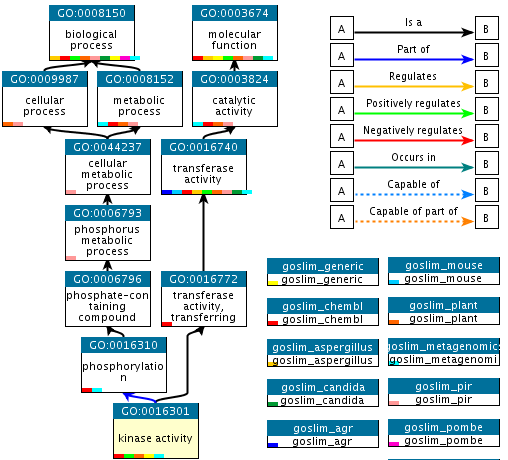
\includegraphics[width=0.8\linewidth]{img/kinase.png}
  \caption{Struktura ontologije}
  \label{fig:kinase}
\end{figure}

Svaka veza(relacija) ima strogo definisana pravila kompozicije koja omogućavaju
automatsko rezonovanje. Recimo relacija \keyword{is\_a} ima svojstvo
tranzitivnosti\parencite{is_a}:
\begin{verbatim}
  A is_a    B  /\  B is_A C   =>    A is_a    C           
  A part_of B  /\  B is_A C   =>    A part_of C
\end{verbatim}

Siže pravila rezonovanja prikazano je na slici \ref{fig:relations}. Ontologije su
dostupne u nekoliko formata. U našem radu korišćen je ravni \file{.obo} format.
Pored njega treba naglasiti postojanje \file{RDF/XML} i \file{OWL} verzija.
Ove verzije namenjene su automatskom rezonovanju unutar specijalizovanih
softvere\footnote{Mi smo koristili Neo4j grafovsku bazu što naš postupak
rezonovanja čini eksplicitnim} i upitnih jezika (protégé, SPARQL, ...).

\begin{figure}[h!]
  \centering
  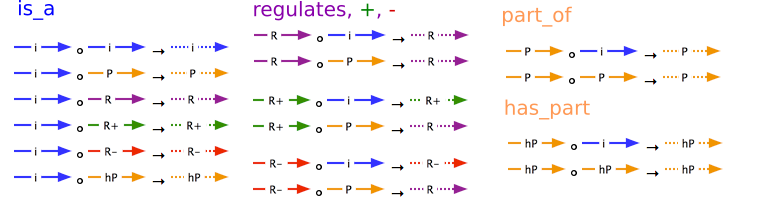
\includegraphics[width=1.0\linewidth]{relations.png}
  \caption{Pravila rezonovanja (isprekidane relacije su rezultat)}
  \label{fig:relations}
\end{figure}

GO termin može biti zastareo u kom slučaju se relacijom \keyword{replaced\_by}
pokazuje na noviji termin. Relacija \keyword{consider} ukazuju na
postojanje mogućih ekvivalentnih termina. Pored glavnog univerzuma postoje i
podskupovi \footnote{Uglavnom ovi podskupovi predstavljaju model organizme}
termina (GO slim) prikazani u donjem desnom delu slike \ref{fig:kinase}.


\subsection{molekulska funkcija}
to say something \parencite{go_mf}




















